\documentclass{ximera}

\input{../preamble.tex}



\title{4.3 - Derivatives of Exponential Functions}

\begin{document}
\begin{abstract}
  We derive the derivative of the natural exponential function and use it to differentiate all exponential functions.
\end{abstract}
\maketitle

We don't have any derivative rules so far that help us compute the derivative of an exponential function, so we go back to the limit definition of the derivative and compute:
\begin{explanation}
\begin{align*}
\ddx a^x &=\lim_{h\to 0} \frac{a^{x+h}-a^x}{h} \\
&=\lim_{h\to 0} \frac{a^xa^{h}-a^x}{h} \\
&=\lim_{h\to 0} a^x\frac{\answer[given]{a^{h}-1}}{h} \\
&=a^x\lim_{h\to 0} \frac{a^{h}-1}{h} \\
&=a^x \cdot \underbrace{\text{(constant)}}_{\lim_{h\to 0} \frac{a^{h}-1}{h}}
\end{align*}
\end{explanation}
There are two interesting things to note here: We are left with a
limit that involves $h$ but not $x$, which means that $
\lim_{h\to 0} (a^h-1)/h$ is a constant. This means that $a^x$ has a remarkable property:
\begin{quote}
  \textbf{The derivative of an exponential function is a constant
    times itself.}
\end{quote}
Unfortunately it is beyond the scope of this text to compute the limit
\[
\lim_{h\to 0} \frac{a^h-1}{h}.
\]
However, we can look at some examples. Consider $(2^h-1)/h$ and $(3^h-1)/h$:

\begin{image}
  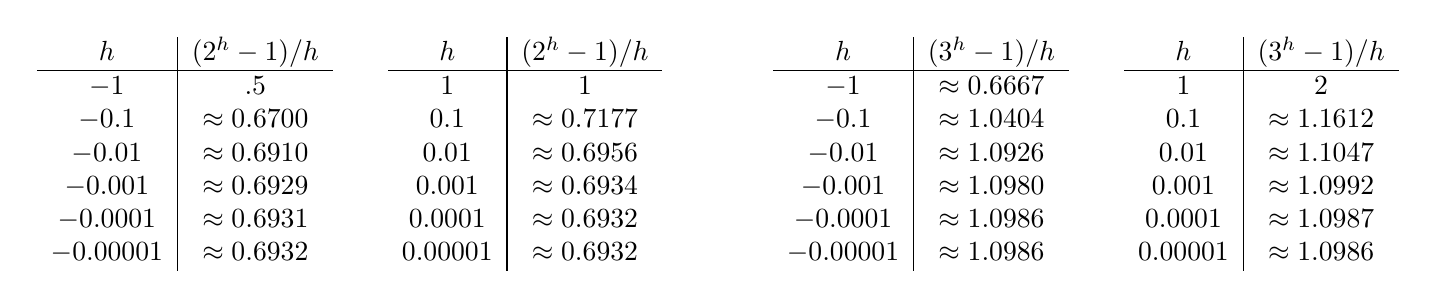
\begin{tikzpicture}
    \node at (0,0) {$\begin{array}{c|c}
 h &     (2^h-1)/h\\ \hline
 -1 & .5  \\
-0.1 &  \approx0.6700 \\
-0.01 & \approx0.6910 \\
-0.001 & \approx0.6929 \\
-0.0001 & \approx0.6931 \\
-0.00001 & \approx0.6932 \\
\end{array}
\qquad
\begin{array}{c|c}
 h &     (2^h-1)/h\\ \hline
 1 & 1  \\
 0.1 &  \approx0.7177 \\
 0.01 & \approx0.6956 \\
 0.001 & \approx0.6934 \\
 0.0001 & \approx0.6932 \\
 0.00001 & \approx0.6932 \\
\end{array}
\qquad\qquad
\begin{array}{c|c}
 h &     (3^h-1)/h\\ \hline
-1 & \approx 0.6667  \\
-0.1 &  \approx1.0404  \\
-0.01 & \approx1.0926 \\
-0.001 & \approx1.0980 \\
-0.0001 & \approx1.0986 \\
-0.00001 & \approx1.0986 \\
\end{array}
\qquad
\begin{array}{c|c}
 h &     (3^h-1)/h\\ \hline
 1 & 2  \\
 0.1 &  \approx1.1612 \\
 0.01 & \approx1.1047 \\
 0.001 & \approx1.0992 \\
 0.0001 & \approx1.0987 \\
 0.00001 & \approx1.0986 \\
 \end{array}$};
\end{tikzpicture}
\end{image}



While these tables don't prove that we have a pattern, it turns out that
\[
\lim_{h\to 0}\frac{2^h-1}{h} \approx .7 \qquad\text{and}\qquad \lim_{h\to 0} \frac{3^h-1}{h} \approx 1.1.
\]
Moreover, if you do more examples, choosing other values for the 
base $a$, you will find that the limit varies
directly with the value of $a$: bigger $a$, bigger limit; smaller $a$,
smaller limit. As we can already see, some of these limits will be
less than $1$ and some larger than $1$. Somewhere between $a=2$ and $a=3$
the limit will be exactly $1$. This happens when 
\[
a = e = 2.718281828459045\dots.
\]
This is in fact the origin of the number $e$ (or at least, one possible origin). We define it by this property:
\begin{definition}\index{e@$e$}
  The number denoted by $e$, called \dfn{Euler's number}, is defined
  to be the number satisfying the following relation
  \[
  \lim_{h\to 0} \frac{e^h-1}{h} = 1.
  \]
\end{definition}
Using this definition, we see that the function $e^x$ has the following truly remarkable property.

\begin{theorem}[The derivative of the natural exponential function]\index{ex@$e^x$}\index{derivative!of ex@of $e^x$}
The derivative of the natural exponential function is itself. That is to say,
\[
\ddx e^x = e^x.
\]
\begin{explanation}  
From the limit definition of the derivative, write
\begin{align*}
\ddx e^x&=\lim_{h\to 0} \frac{e^{x+h}-e^x}{h} \\
&=\lim_{h\to 0} \frac{e^xe^{h}-e^x}{h} \\
&=\lim_{h\to 0} \answer[given]{e^x}\frac{e^{h}-1}{h} \\
&=e^x\lim_{h\to 0} \frac{e^{h}-1}{h} \\
&=e^x.
\end{align*}
\end{explanation}
\end{theorem}


Hence $e^x$ is its own derivative. In other words, the function $f(x)=e^x$ goes through the point $(a,e^a)$ with slope $e^a$ at that point, no matter what $a$ is. 

\begin{question}
  What is the slope of the tangent line to the function $f(x) = e^x$ at $x = 5$?
  \begin{prompt}
    The slope is $\answer{e^5}$.
  \end{prompt}
\end{question}



\begin{example}
Compute:
\[
\ddx\left(8\sqrt{x} + 7e^x \right)
\]
	\begin{explanation}
		Write with me:
		\begin{align*}
			\ddx\left(8\sqrt{x} + 7e^x \right) &= 8\ddx x^{1/2} + 7\ddx e^x\\
				&= 4x^{-1/2} + 7 \answer[given]{e^x}.
		\end{align*}
	\end{explanation}
\end{example}




\begin{example}
	Compute: \[ \ddx e^{4x\sqrt{x+1}} \]
	\begin{explanation}
		Notice that $e^{4x \sqrt{x+1}}$ is a composition $f(g(x))$ with $f(x) = e^x$ and $g(x) = 4x \sqrt{x+1}$. To differentiate a composition, we use the chain rule: 
		$$\ddx f(g(x)) = f'( g(x) ) g'(x).$$  
		
		We know $f'(x) = \ddx e^x = e^x$ and $g'(x) = \ddx \left( 4x \sqrt{x+1} \right)$ which we calculate by product rule as
		$4 \sqrt{x+1} + 4x \dfrac{1}{2 \sqrt{x+1}} \cdot 1$ (where we used chain rule AGAIN inside the square root).
		Our answer is then:
		\[ e^{4x \sqrt{x+1}}\left( 4\sqrt{x+1} + \dfrac{2x}{\sqrt{x+1}}\right).\]
	\end{explanation}	
\end{example}

\begin{question}
	  Find $\displaystyle \eval{\ddx \left(x^{4/3}+\frac{7}{3}\right) e^{2x}}_{x=0}$.
	  
  \begin{prompt}
    \[\displaystyle \eval{\ddx \left(x^{4/3}+\frac{7}{3}\right) e^{2x}}_{x=0} = \answer{\frac{14}{3}}.\]
  \end{prompt}
\end{question}




\section{The Derivative of Other Exponentials}
Remember that any number $b > 0$ can be written in the form $e^x$ for some specific value of $x$. For any base $b$, we can write:
\begin{align*}
	b^x &= (b)^x\\
		&= \left( e^{\ln b} \right)^x\\
		&= e^{x \ln b}.
\end{align*}

Thus to compute $\ddx b^x$ we can see $b^x$ as a composition and use the chain rule:
\begin{align*} 
	\ddx b^x &= \ddx e^{x \ln b}\\
		&= e^{x \ln b} \cdot \ddx \left( x \ln b \right)\\ 
		&= e^{x \ln b} \cdot (\ln b).
\end{align*}
Rewriting $e^{x \ln b}$ as $b^x$ we get $b^x\ln b$.
\begin{theorem}
	The derivative of the exponential function $b^x$, for $b > 0$, $b \neq 1$ is given by:
	\[ \ddx b^x = b^x \ln b. \]
\end{theorem}

\begin{example}
	Compute $\displaystyle \ddx 7^x$.
	\begin{explanation}
		Using our new derivative rule with $b = 7$, we get  $\displaystyle 7^x \ln 7$.
	\end{explanation}
\end{example}

\begin{example}
	Compute $\displaystyle \ddx \left(\frac{2}{3}\right)^x$.
	\begin{explanation}
		Using our new derivative rule with $b = 2/3$, we get  $\displaystyle \left(\frac{2}{3}\right)^x \ln \frac{2}{3}$.
	\end{explanation}
\end{example}

\begin{example}
	Compute $\displaystyle \ddx 3^{x^2+2x}$.
	\begin{explanation}
		This is a composition $f(g(x))$ with $f(x)=3^x$ and $g(x)=x^2+2x$, so we use the chain rule:
		\begin{align*}
			\ddx 3^{x^2 + 2x} &= 3^{\answer[given]{x^2+2x}} \cdot \ln \left( \answer[given]{3} \right) \cdot \ddx \left(  \answer[given]{x^2+2x}\right)\\
				&= 3^{x^2+2x} \ln(3) (2x+2).
		\end{align*}
	\end{explanation}
\end{example}


\subsection{Learning Objectives}
After completing this section, students should be able to:
\vspace{.05in}

\noindent$\bullet$ Differentiate $b^x$ for any base $b$.
\\$\bullet$ Compute derivatives involving products, quotients, and/or compositions involving exponential functions.





%\outcome{Use ``shortcut'' rules to find and use derivatives.}
%\outcome{Use the definition of the derivative to develop a shortcu rule to find the derivative of the natural exponential function.}

\end{document}